% ===========================================================================
%  Pokedex Tutorial — Casual User Guide (LaTeX)
%  Created: 2026-07-07
%  Last modified: 2026-07-07
%  Description: A printable, beginner-friendly guide to using the Pokedex app.
%               Covers installation, basic usage, and troubleshooting.
%               Compatible with basic TeX Live distribution (no extra packages).
%  Author: enigmak9
% ===========================================================================

\documentclass[11pt,a4paper]{article}

% ── Packages (basic distribution only) ──────────────────────────────────────
\usepackage[utf8]{inputenc}
\usepackage[T1]{fontenc}
\usepackage{geometry}
\usepackage{hyperref}
\usepackage{graphicx}
\usepackage{color}
\usepackage{fancyhdr}
\usepackage{listings}
\usepackage{tikz}
\usepackage{booktabs}

% ── Page Setup ──────────────────────────────────────────────────────────────
\geometry{margin=1in, bottom=1.2in}
\hypersetup{
    colorlinks=true,
    linkcolor=blue!60!black,
    urlcolor=blue!60!black,
    citecolor=blue!60!black
}

% ── Colors ──────────────────────────────────────────────────────────────────
\definecolor{pokedexred}{rgb}{0.86, 0.08, 0.24}
\definecolor{pokedexblue}{rgb}{0.12, 0.56, 1.00}
\definecolor{pokedexgreen}{rgb}{0.13, 0.55, 0.13}
\definecolor{codebg}{rgb}{0.96, 0.96, 0.96}
\definecolor{tipframe}{rgb}{0.40, 0.60, 0.80}
\definecolor{warnframe}{rgb}{1.00, 0.65, 0.00}
\definecolor{tipbg}{rgb}{0.95, 0.98, 1.00}
\definecolor{warnbg}{rgb}{1.00, 0.98, 0.90}

% ── Header / Footer ─────────────────────────────────────────────────────────
\pagestyle{fancy}
\fancyhf{}
\fancyhead[L]{\small\textbf{Pok\'{e}dex Tutorial — Casual User Guide}}
\fancyhead[R]{\small\thepage}
\fancyfoot[C]{\small\textit{Keep exploring!}}
\renewcommand{\headrulewidth}{0.4pt}

% ── Custom Environments ─────────────────────────────────────────────────────
% Simple framed box for tips (replaces tcolorbox)
\newenvironment{tipbox}
{\vspace{10pt}\noindent\colorbox{tipbg}{\begin{minipage}{0.95\textwidth}\textbf{Tip:} }
{\end{minipage}}\vspace{10pt}}

\newenvironment{warnbox}
{\vspace{10pt}\noindent\colorbox{warnbg}{\begin{minipage}{0.95\textwidth}\textbf{Note:} }
{\end{minipage}}\vspace{10pt}}

% Tight itemize/enumerate spacing (replaces enumitem)
\newenvironment{tightitemize}
{\begin{itemize}\setlength{\itemsep}{2pt}\setlength{\parskip}{0pt}}
{\end{itemize}}

\newenvironment{tightenumerate}
{\begin{enumerate}\setlength{\itemsep}{2pt}\setlength{\parskip}{0pt}}
{\end{enumerate}}

% ── Code Style ──────────────────────────────────────────────────────────────
\lstdefinestyle{bashstyle}{
    backgroundcolor=\color{codebg},
    basicstyle=\ttfamily\footnotesize,
    breaklines=true,
    frame=single,
    numbers=none,
    xleftmargin=8pt,
    xrightmargin=8pt
}

% ── Title ───────────────────────────────────────────────────────────────────
\title{
    \textbf{\Huge Pok\'{e}dex Tutorial}\\[4pt]
    \large A Casual User's Guide to Building and Using the App\\[8pt]
    \normalsize Version 1.0 — July 2026
}
\author{enigmak9}
\date{}

\begin{document}

\maketitle
\thispagestyle{fancy}

% ── Abstract ────────────────────────────────────────────────────────────────
\begin{center}
\fbox{
\begin{minipage}{0.85\textwidth}
\small
\textbf{About this guide:} This document is for \textit{casual users} — people who want to run the app, understand what it does, and maybe tweak a few settings. It assumes very basic familiarity with computers. If you're comfortable with the command line, also see \texttt{docs/run.md}. If you want to modify the code, start with \texttt{docs/architecture.md}.
\end{minipage}
}
\end{center}

\tableofcontents
\newpage

% ═══════════════════════════════════════════════════════════════════════════
%  SECTION 1: WHAT IS THIS?
% ═══════════════════════════════════════════════════════════════════════════
\section{What Is This App?}

The \textbf{Pok\'{e}dex Tutorial} is an iOS app that acts like a Pok\'{e}dex — an encyclopedia of Pok\'{e}mon creatures. You can:

\begin{tightitemize}
    \item \textbf{Browse} all 1,300+ Pok\'{e}mon, with official artwork
    \item \textbf{Search} for any Pok\'{e}mon by name
    \item \textbf{Filter} by type (Fire, Water, Grass, etc.)
    \item \textbf{View details}: base stats, abilities, type effectiveness
    \item \textbf{Save favorites} for quick access
    \item \textbf{Switch} between list and grid layouts
\end{tightitemize}

But this app is also a \textbf{teaching tool}. Every file is heavily commented to explain \textit{why} the code is written the way it is. It is designed to teach modern iOS development with Swift and SwiftUI, from basic types to advanced networking and testing.

\begin{tipbox}
\textbf{New to Swift?} Start by reading the comments in \texttt{PokedexTutorial/Models/Pokemon.swift}. It walks through structs, protocols, and JSON decoding step by step. Then move to \texttt{PokemonListView.swift} to see how the UI connects.
\end{tipbox}

% ═══════════════════════════════════════════════════════════════════════════
%  SECTION 2: GETTING STARTED
% ═══════════════════════════════════════════════════════════════════════════
\section{Getting Started}

\subsection{What You Need}

\begin{tightitemize}
    \item A Mac computer running \textbf{macOS 14 (Sonoma)} or newer
    \item \textbf{Xcode 15.2} or newer (free from the Mac App Store)
    \item An internet connection (for live Pok\'{e}mon data)
    \item About 200 MB of free disk space
\end{tightitemize}

\subsection{Opening the Project}

\begin{tightenumerate}
    \item Locate the \texttt{swift-pokedex-tutorial} folder on your Mac.
    \item Double-click the file named \texttt{PokedexTutorial.xcodeproj}.\\
          \textit{(It has a blue icon with a hammer.)}
    \item Xcode will open. Wait a moment while it indexes the files.
    \item At the top-left of Xcode, you'll see a device selector. Click it and choose any iPhone simulator (e.g., ``iPhone 17 Pro'').
\end{tightenumerate}

\subsection{Running the App}

\begin{tightenumerate}
    \item Press \textbf{Cmd + R} (hold the Command key and press R).
    \item Xcode will build the app. The first build takes 30--60 seconds.
    \item The Simulator opens automatically. The app appears and loads the Pok\'{e}mon list from the internet.
\end{tightenumerate}

\begin{tipbox}
\textbf{First build taking too long?} That's normal. Xcode is compiling all the Swift files. Subsequent builds are much faster (5--15 seconds).
\end{tipbox}

\subsection{Running Without Internet}

If you don't have internet, you can use local mock data:

\begin{tightenumerate}
    \item In Xcode, open \texttt{PokedexTutorial/App/PokedexTutorialApp.swift}.
    \item Find the line that says:\\[4pt]
          \texttt{@StateObject private var pokemonService: PokemonAPIService =}\\
          \hspace{20pt}\texttt{PokemonAPIService()}
    \item Replace it with:\\[4pt]
          \texttt{@StateObject private var pokemonService = MockPokemonService()}
    \item Press Cmd + R to rebuild. The app now shows 10 sample Pok\'{e}mon instantly.
\end{tightenumerate}

% ═══════════════════════════════════════════════════════════════════════════
%  SECTION 3: USING THE APP
% ═══════════════════════════════════════════════════════════════════════════
\section{Using the App}

\subsection{The Main Screen}

When you launch the app, you see:

\begin{center}
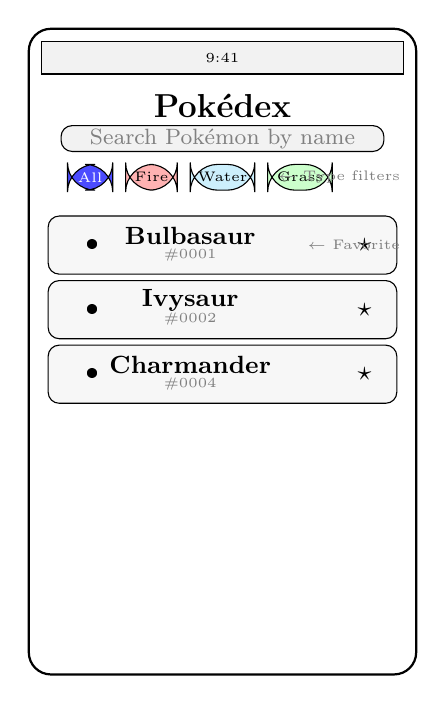
\begin{tikzpicture}[scale=0.82]
    % Phone frame
    \draw[thick, rounded corners=8pt] (0,0) rectangle (6,10);
    % Status bar
    \draw[fill=black!5] (0.2,9.3) rectangle (5.8,9.8);
    \node at (3,9.55) {\tiny 9:41};
    % Title
    \node[font=\large\bfseries] at (3,8.8) {Pok\'{e}dex};
    % Search bar
    \draw[fill=black!5, rounded corners=4pt] (0.5,8.1) rectangle (5.5,8.5);
    \node[font=\footnotesize, text=gray] at (3,8.3) {Search Pok\'{e}mon by name};
    % Type chips
    \draw[fill=blue!70, rounded corners=10pt] (0.6,7.5) rectangle (1.3,7.9);
    \node[font=\tiny, text=white] at (0.95,7.7) {All};
    \draw[fill=red!30, rounded corners=10pt] (1.5,7.5) rectangle (2.3,7.9);
    \node[font=\tiny] at (1.9,7.7) {Fire};
    \draw[fill=cyan!20, rounded corners=10pt] (2.5,7.5) rectangle (3.5,7.9);
    \node[font=\tiny] at (3.0,7.7) {Water};
    \draw[fill=green!20, rounded corners=10pt] (3.7,7.5) rectangle (4.7,7.9);
    \node[font=\tiny] at (4.2,7.7) {Grass};
    % Row 1
    \draw[fill=black!3, rounded corners=4pt] (0.3,6.2) rectangle (5.7,7.1);
    \node at (1.0,6.65) {\small\textbullet};
    \node[font=\small\bfseries] at (2.5,6.8) {Bulbasaur};
    \node[font=\tiny, text=gray] at (2.5,6.5) {\#0001};
    % Row 2
    \draw[fill=black!3, rounded corners=4pt] (0.3,5.2) rectangle (5.7,6.1);
    \node at (1.0,5.65) {\small\textbullet};
    \node[font=\small\bfseries] at (2.5,5.8) {Ivysaur};
    \node[font=\tiny, text=gray] at (2.5,5.5) {\#0002};
    % Row 3
    \draw[fill=black!3, rounded corners=4pt] (0.3,4.2) rectangle (5.7,5.1);
    \node at (1.0,4.65) {\small\textbullet};
    \node[font=\small\bfseries] at (2.5,4.8) {Charmander};
    \node[font=\tiny, text=gray] at (2.5,4.5) {\#0004};
    % Star buttons
    \node at (5.2,6.65) {$\star$};
    \node at (5.2,5.65) {$\star$};
    \node at (5.2,4.65) {$\star$};
    % Labels
    \node[font=\tiny, text=gray, anchor=east] at (5.9,7.7) {$\leftarrow$ Type filters};
    \node[font=\tiny, text=gray, anchor=east] at (5.9,6.65) {$\leftarrow$ Favorite};
\end{tikzpicture}
\end{center}

\subsubsection{Key Interactions}

\begin{description}
    \item[\textbf{Scroll down}] to see more Pok\'{e}mon. The app loads 20 at a time (infinite scroll).
    \item[\textbf{Pull down}] from the top to refresh the list with fresh data.
    \item[\textbf{Tap the search bar}] at the top and type a Pok\'{e}mon name. The list filters as you type.
    \item[\textbf{Tap a type chip}] (Fire, Water, Grass, etc.) to show only Pok\'{e}mon of that type. Tap ``All'' to clear the filter.
    \item[\textbf{Tap the star} $\star$] on any row to mark it as a favorite.
    \item[\textbf{Tap the star button}] in the toolbar (top-right) to show only your favorites.
    \item[\textbf{Tap the grid button}] (four squares icon) to switch between list and grid layout.
    \item[\textbf{Tap any Pok\'{e}mon}] to see its full details.
\end{description}

\subsection{The Detail Screen}

When you tap a Pok\'{e}mon, you see:

\begin{center}
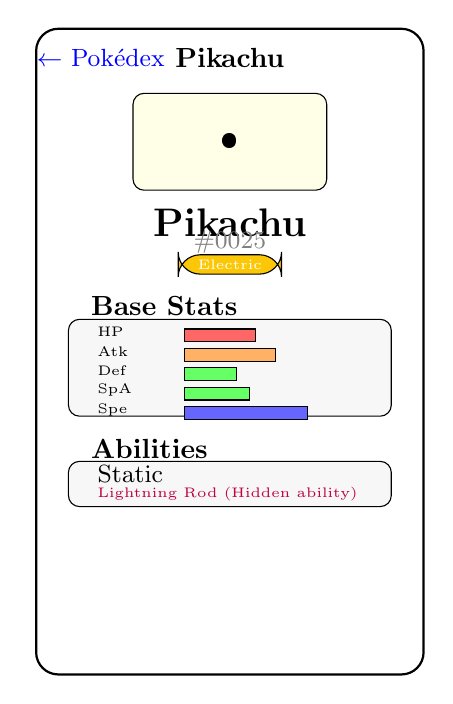
\begin{tikzpicture}[scale=0.82]
    \draw[thick, rounded corners=8pt] (0,0) rectangle (6,10);
    % Back button
    \node[font=\small, text=blue] at (1.0,9.55) {$\leftarrow$ Pok\'{e}dex};
    % Title
    \node[font=\bfseries] at (3,9.55) {Pikachu};
    % Artwork area
    \draw[fill=yellow!10, rounded corners=4pt] (1.5,7.5) rectangle (4.5,9.0);
    \node at (3,8.25) {\Large\textbullet};
    % Name & number
    \node[font=\Large\bfseries] at (3,7.0) {Pikachu};
    \node[font=\small, text=gray] at (3,6.7) {\#0025};
    % Type badge
    \draw[fill=yellow!60!orange, rounded corners=8pt] (2.2,6.2) rectangle (3.8,6.5);
    \node[font=\tiny, text=white] at (3,6.35) {Electric};
    % Stats section
    \node[font=\bfseries, anchor=west] at (0.7,5.7) {Base Stats};
    \draw[fill=black!3, rounded corners=4pt] (0.5,4.0) rectangle (5.5,5.5);
    \node[font=\tiny, anchor=west] at (0.8,5.3) {HP};
    \draw[fill=red!60] (2.3,5.15) rectangle (3.4,5.35);
    \node[font=\tiny, anchor=west] at (0.8,5.0) {Atk};
    \draw[fill=orange!60] (2.3,4.85) rectangle (3.7,5.05);
    \node[font=\tiny, anchor=west] at (0.8,4.7) {Def};
    \draw[fill=green!60] (2.3,4.55) rectangle (3.1,4.75);
    \node[font=\tiny, anchor=west] at (0.8,4.4) {SpA};
    \draw[fill=green!60] (2.3,4.25) rectangle (3.3,4.45);
    \node[font=\tiny, anchor=west] at (0.8,4.1) {Spe};
    \draw[fill=blue!60] (2.3,3.95) rectangle (4.2,4.15);
    % Abilities section
    \node[font=\bfseries, anchor=west] at (0.7,3.5) {Abilities};
    \draw[fill=black!3, rounded corners=4pt] (0.5,2.6) rectangle (5.5,3.3);
    \node[font=\small, anchor=west] at (0.8,3.1) {Static};
    \node[font=\tiny, text=purple, anchor=west] at (0.8,2.8) {Lightning Rod (Hidden ability)};
\end{tikzpicture}
\end{center}

\subsubsection{Detail Screen Features}

\begin{tightitemize}
    \item \textbf{Official artwork} at the top, on a tinted background matching the Pok\'{e}mon's type
    \item \textbf{Base stats} with color-coded bars: red (low), orange (medium), green (high), blue (exceptional)
    \item \textbf{Abilities} listed below stats; hidden abilities are marked in purple
    \item \textbf{Type Effectiveness} (expandable section, tap to open) shows what types the Pok\'{e}mon is weak to, resistant to, and immune to
    \item \textbf{Star button} in the toolbar to favorite/unfavorite
\end{tightitemize}

\begin{warnbox}
Type effectiveness data loads \textit{only} when you expand the section. This is deliberate — it avoids unnecessary network calls for information you might not need.
\end{warnbox}

% ═══════════════════════════════════════════════════════════════════════════
%  SECTION 4: FAVORITES
% ═══════════════════════════════════════════════════════════════════════════
\section{Favorites Explained}

Favorites are saved \textbf{even after you close the app}. They are stored on your Mac using a technology called UserDefaults.

\begin{tightitemize}
    \item \textbf{Add a favorite:} Tap the $\star$ (star) icon on any Pok\'{e}mon row. It turns yellow.
    \item \textbf{Remove a favorite:} Tap the yellow $\star$ again. It turns gray.
    \item \textbf{View only favorites:} Tap the star button in the toolbar (top-right corner). Tap again to show all.
    \item \textbf{Favorites survive restarts:} Close and reopen the app — your favorites are still there.
\end{tightitemize}

\begin{tipbox}
Favorites are stored as a simple list of Pok\'{e}mon IDs. This means they work offline and load instantly. If you uninstall the app, favorites are lost (they're stored locally, not in the cloud).
\end{tipbox}

% ═══════════════════════════════════════════════════════════════════════════
%  SECTION 5: TROUBLESHOOTING
% ═══════════════════════════════════════════════════════════════════════════
\section{Troubleshooting}

\subsection{The app shows a loading spinner forever}

This usually means the Pok\'{e}API (free service we use for data) is unavailable or your internet is down.

\begin{tightenumerate}
    \item Check your internet connection.
    \item Wait a minute — the Pok\'{e}API has rate limits. Too many rapid requests will be blocked temporarily.
    \item Switch to mock data: edit \texttt{PokedexTutorialApp.swift} to use \texttt{MockPokemonService()} instead of \texttt{PokemonAPIService()}.
\end{tightenumerate}

\subsection{The app shows ``No Pok\'{e}mon Found''}

You may have an active search or filter that matches nothing.

\begin{tightenumerate}
    \item Clear the search bar (tap the \textbf{X} button or delete all text).
    \item Make sure the ``All'' type chip is selected (it should be filled, not outlined).
    \item If the star filter is active (yellow star in toolbar), tap it to show all Pok\'{e}mon.
\end{tightenumerate}

\subsection{Xcode says ``Build Failed''}

\begin{tightenumerate}
    \item Make sure you're opening \texttt{PokedexTutorial.xcodeproj}, not individual \texttt{.swift} files.
    \item In Xcode, go to \textbf{Product} $\rightarrow$ \textbf{Clean Build Folder} (hold Option key to see this), then try building again.
    \item Make sure your selected simulator is running iOS 17.0 or newer.
    \item Check that Xcode is version 15.2 or newer (Apple menu $\rightarrow$ About Xcode).
\end{tightenumerate}

\subsection{Tests fail with network errors}

The API tests need an internet connection. If they fail:

\begin{tightenumerate}
    \item Check your internet connection.
    \item Run them again — the Pok\'{e}API may have been temporarily rate-limiting.
    \item All other tests (model tests, ViewModel tests) pass without internet.
\end{tightenumerate}

% ═══════════════════════════════════════════════════════════════════════════
%  SECTION 6: LEARNING PATH
% ═══════════════════════════════════════════════════════════════════════════
\section{Learning Path}

This app is designed to teach Swift and iOS development. Here's the recommended reading order:

\begin{tightenumerate}
    \item \textbf{Start here:} \texttt{Models/Pokemon.swift}\\
          Learn structs, protocols (Codable, Identifiable, Hashable), computed properties, and custom JSON decoding.

    \item \textbf{Then:} \texttt{Models/PokemonType.swift}\\
          Understand enums with associated values, CaseIterable, and how to attach display data (colors, icons) to enum cases.

    \item \textbf{MVVM pattern:} \texttt{ViewModels/PokemonListViewModel.swift}\\
          See how @Published, @MainActor, ObservableObject, and Combine work together to manage UI state.

    \item \textbf{Networking:} \texttt{Services/PokemonAPIService.swift}\\
          Learn async/await, URLSession, Codable decoding, and typed error handling with a custom error enum.

    \item \textbf{SwiftUI basics:} \texttt{Views/PokemonRowView.swift} and \texttt{Views/TypeBadgeView.swift}\\
          Understand view composition, AsyncImage, @EnvironmentObject, and accessibility.

    \item \textbf{SwiftUI advanced:} \texttt{Views/PokemonListView.swift}\\
          Study NavigationStack, .searchable, .refreshable, infinite scroll, LazyVGrid, and value-based navigation.

    \item \textbf{Custom layouts:} \texttt{Views/PokemonDetailView.swift}\\
          Learn the Layout protocol, GeometryReader, and async state handling.

    \item \textbf{Testing:} \texttt{PokedexTutorialTests/}\\
          See how to write unit tests with XCTest using the AAA pattern with mock services.
\end{tightenumerate}

\begin{tipbox}
\textbf{Study tip:} Read each file \textit{top to bottom}. The comments form a narrative. Don't skip the header comment — it explains the file's role in the architecture.
\end{tipbox}

% ═══════════════════════════════════════════════════════════════════════════
%  SECTION 7: COMMAND LINE QUICK REFERENCE
% ═══════════════════════════════════════════════════════════════════════════
\section{Command Line Quick Reference}

For users comfortable with Terminal:

\begin{lstlisting}[style=bashstyle]
# Build the app
xcodebuild -project PokedexTutorial.xcodeproj \
  -scheme PokedexTutorial \
  -destination 'platform=iOS Simulator,name=iPhone 17 Pro' \
  build

# Run all tests (24 tests, ~2 seconds)
xcodebuild -project PokedexTutorial.xcodeproj \
  -scheme PokedexTutorial \
  -destination 'platform=iOS Simulator,name=iPhone 17 Pro' \
  test

# Launch in simulator
xcrun simctl boot "iPhone 17 Pro"
xcrun simctl install "iPhone 17 Pro" \
  ~/Library/Developer/Xcode/DerivedData/PokedexTutorial-*/Build/Products/Debug-iphonesimulator/PokedexTutorial.app
xcrun simctl launch "iPhone 17 Pro" com.enigmak9.PokedexTutorial

# Open in Xcode
open PokedexTutorial.xcodeproj
\end{lstlisting}

% ═══════════════════════════════════════════════════════════════════════════
%  SECTION 8: PROJECT STRUCTURE REFERENCE
% ═══════════════════════════════════════════════════════════════════════════
\section{Project Structure Reference}

\begin{center}
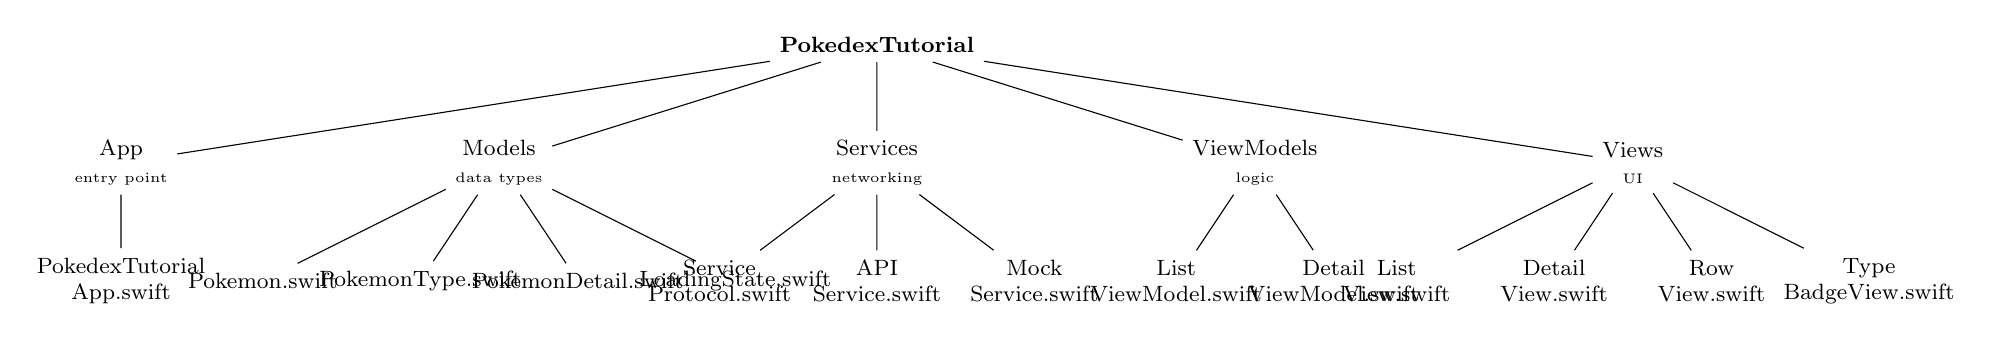
\begin{tikzpicture}[
    level 1/.style={sibling distance=48mm},
    level 2/.style={sibling distance=20mm},
    every node/.style={font=\footnotesize, align=center}
]
\node {\textbf{PokedexTutorial}}
    child { node {App\\\tiny entry point}
        child { node {PokedexTutorial\\App.swift} }
    }
    child { node {Models\\\tiny data types}
        child { node {Pokemon.swift} }
        child { node {PokemonType.swift} }
        child { node {PokemonDetail.swift} }
        child { node {LoadingState.swift} }
    }
    child { node {Services\\\tiny networking}
        child { node {Service\\Protocol.swift} }
        child { node {API\\Service.swift} }
        child { node {Mock\\Service.swift} }
    }
    child { node {ViewModels\\\tiny logic}
        child { node {List\\ViewModel.swift} }
        child { node {Detail\\ViewModel.swift} }
    }
    child { node {Views\\\tiny UI}
        child { node {List\\View.swift} }
        child { node {Detail\\View.swift} }
        child { node {Row\\View.swift} }
        child { node {Type\\BadgeView.swift} }
    };
\end{tikzpicture}
\end{center}

% ═══════════════════════════════════════════════════════════════════════════
%  APPENDIX: KEYBOARD SHORTCUTS (SIMULATOR)
% ═══════════════════════════════════════════════════════════════════════════
\section*{Appendix: Simulator Keyboard Shortcuts}

\begin{center}
\begin{tabular}{ll}
\toprule
\textbf{Shortcut} & \textbf{Action} \\
\midrule
Cmd + 1 & 100\% scale (actual size) \\
Cmd + 2 & 75\% scale \\
Cmd + 3 & 50\% scale \\
Cmd + 4 & 33\% scale \\
Cmd + 5 & 25\% scale \\
Cmd + K & Toggle software keyboard \\
Cmd + Shift + H & Go to Home screen \\
Cmd + Shift + H H & App switcher (double-press) \\
Cmd + Left/Right & Rotate device \\
\bottomrule
\end{tabular}
\end{center}

% ═══════════════════════════════════════════════════════════════════════════
%  FINAL PAGE
% ═══════════════════════════════════════════════════════════════════════════
\vfill
\begin{center}
\rule{0.5\textwidth}{0.4pt}\\[8pt]
{\small
\textit{This guide was written as part of the Pok\'{e}dex Tutorial project.}\\
\textit{For technical documentation, see \texttt{docs/architecture.md} and \texttt{docs/flowcharts.md}.}\\
\textit{For the quick-start guide, see \texttt{docs/run.md}.}\\[4pt]
\textbf{Questions?} Open an issue in the repository.\\[4pt]
Created by \textbf{enigmak9} • July 2026
}
\end{center}

\end{document}
